\section{Esercitazione capitoli 1 e 2}
\subsection{A.A. 2022/23}
\begin{enumerate}
    \item Approssimando $\pi = 3.14159265\hdots$ con $3.14$:
        \begin{itemize}
            \item qual è l’errore assoluto commesso?
            \item  qual è quello relativo?
        \end{itemize}
        (approssimare la risposta a due cifre significative).
        \item Come si definisce la precisione di macchina di un’aritmetica finita? Qual è il suo significato?
        \item Qual è la precisione di macchina della singola e doppia precisione IEEE? Dedurre il numero di cifre decimali approssimativamente disponibili per la mantissa.
        \item Cosa è il fenomeno della cancellazione numerica?
        \item Come si definisce l’ordine di convergenza di un metodo per la ricerca degli zeri di una funzione?
        \item Qual è il numero massimo di iterazioni che richiederà il metodo di bisezione per determinare la radice di una funzione assegnata con tolleranza (assoluta) $10^{-3}$, se l’intervallo di confidenza iniziale è $[33, 37]$?
        \item Derivare il metodo di Newton per la ricerca della radice di una funzione e dimostrare che esso converge quadraticamente a radici semplici.
        \item Calcolare il numero di condizionamento della radice nulla di
        \begin{equation*}
            f(x)=3e^x-2\cos{x}-1.
        \end{equation*}
        \item Definire la molteplicità di una radice. Calcolare la molteplicità della radice nulla di
        \begin{equation*}
            f(x)=e^{x^2}-1.
        \end{equation*}
        Perché il calcolo di una radice nulla è un problema malcondizionato?
        \item Scrivere una function Matlab che implementi efficientemente il metodo di Newton.
\end{enumerate}

\paragraph{1.}\footnote{Slide 3 PDF 13.} $x = 3.14159265\hdots,\, \Tilde{x}=3.14\Rightarrow\begin{cases}
    |\Delta x|=|\Tilde{x}-x|=0.0015926\hdots\approx 1.6\times 10^{-3},\\
    |\xi_x|=\frac{|\Delta x|}{|x|}=\frac{1.6\times 10^{-3}}{3.1415\hdots}\approx 5\times 10^{-4}.
\end{cases}$

\paragraph{2.}\footnote{Slide 3 PDF 13.} La precisione di macchina di un'aritmetica finita rappresenta una maggiorazione \textbf{uniforme} dell'errore relativo di rappresentazione, per numeri rappresentati da numeri di macchina normalizzati. Se è utilizzata una base $b$, con $m$ cifre per la mantissa, essa vale: $u=\begin{cases}
b^{1-m},\;\text{in caso di rappresentazione con troncamento};\\
\frac{1}{2}b^{1-m},\;\text{in caso di rappresentazione con arrotondamento.}
\end{cases}$

\paragraph{3.}\footnote{Slide 4 PDF 13. Nella rappresentazione binaria le cifre sono normalizzate, tutto cambia se è denormalizzato. La prima cifra considerata 1 quindi non è memorizzata memorizzando con 23 bit 24. Stesso cosa vale per la precisione macchina in doppia precisione.} Nella precisione IEEE è utilizzata la rappresentazione in base 2 con arrotondamento alla 24-esima cifra binaria. Pertanto la precisione di macchina è
\begin{equation*}
   \boldsymbol{u=\frac{1}{2}\cdot 2^{1-24}=2^{-24}}\approx\frac{10^{-6}}{16}\approx\boldsymbol{0.7\cdot 10^{-7}},
\end{equation*}
ovvero, poco più di 7 cifre decimali significative.

\noindent Per la doppia precisione, l'unica differenza consiste nel numero di cifre binarie significative, sono 53. Pertanto, 
\begin{equation*}
    \boldsymbol{u=\frac{1}{2}\cdot 2^{1-53}=2^{-53}\approx 10^{-16}},
\end{equation*}
ovvero, circa 16 cifre decimali.

\paragraph{4.}\footnote{Slide 4 PDF 13.} La cancellazione numerica consiste nella perdita di cifre significative, nel risultato, derivante dalla somma di addendi quasi opposti. Ciò è dovuto al malcondizionamento di questa operazione. Dati $x$ e $y$ numeri da sommare, il numero di condizionamento della somma è rappresentato da $\kappa=\frac{|x|+|y|}{|x+y|}$, il quale non è limitato superiormente se $x\approx -y$. 

\paragraph{5.}\footnote{Slide 5 PDF 13.} Sia $x_{n+1}=\Phi(x_n),\; n=0,1,\hdots,$ denota un generico metodo iterativo per la ricerca di una radice $\overline{x}$ dell'equazione $f(x)=0$. Supposto che $x_n\rightarrow\overline{x}$, per $n\rightarrow\infty$ e con $e_n=|x_n-\overline{x}|$ il corrispondente errore al passo $n$. Il metodo converge con ordine $p\geq 1 $ alla radice, se $p$ è il più grande valore reale per cui 
\begin{equation*}
    \lim_{n\rightarrow\infty}\frac{e_{n+1}}{e_n^p}=c<\infty,
\end{equation*}
dove $c$ è la costante asintotica dell'errore. Per $n>>1\Rightarrow e_{n+1}\approx c\cdot e_n^p$.

\paragraph{6.}\footnote{Slide 6 PDF 13.} Il metodo di bisezione dimezza, ad ogni iterazione, l'ampiezza dell'intervallo di confidenza. Pertanto, l'approssimazione al passo $n$, avrà una accuratezza $2^{-n}(b-a)$, essendo $b-a$ l'ampiezza dell'intervallo iniziale. In questo caso $b-a=4$, per cui è ottenuto, imponendo $2^{2-n}\leq 10^{-3}$, il numero massimo di iterazioni. Dato che $10^{-3}\approx 2^{-10}$ è ottenuto quanto segue: $2^{2-n}\leq 2^{-10}\Rightarrow 2-n\leq -10\Rightarrow n\geq 12 \Rightarrow\boldsymbol{n=12}\, \left(= \lceil\log_2(37-34)-\log_2(10^{-3})\rceil\right)$.

\paragraph{7.}\footnote{Slide 7 PDF 13.} Il metodo di Newton è ottenuto ricercando, ad ogni passo, la radice della retta tangente al grafico della funzione nell'approssimazione corrente (come in Figura \ref{fig:approxNewtEs10}).

\begin{figure}
    \centering
    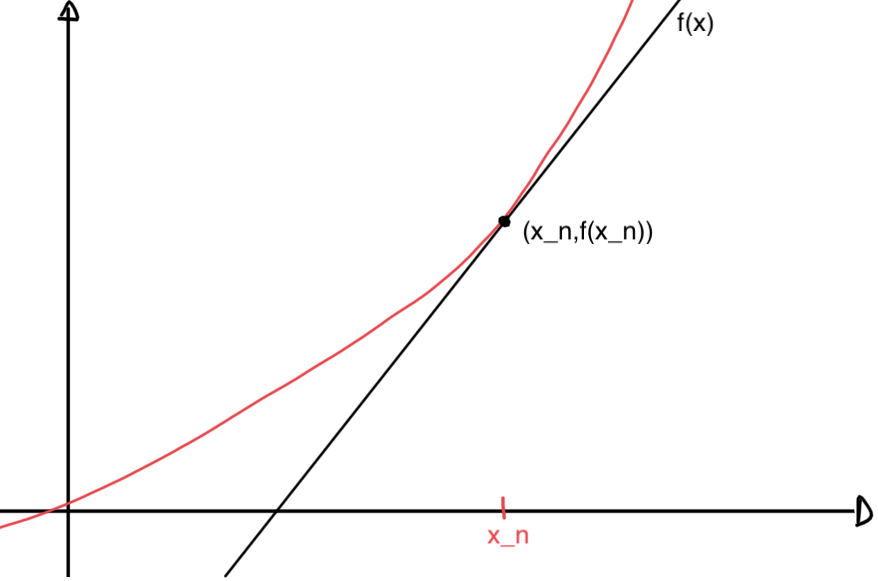
\includegraphics[width=0.5\textwidth]{immagini/approxNewtEs10.jpg}
    \caption{Approssimazione esercizio 10.}\label{fig:approxNewtEs10}
\end{figure}

\noindent La retta tangente il grafico di $f(x)$ nel punto $(x_n, f(x_n))$ è $y-f(x_n)=f'(x_n)(x-x_n)$, essendo $f'(x_n)$ la derivata di $f(x).$ Ponendo $y=0$, è ricavata
\begin{equation*}
    x_{n+1}=x_n-\frac{f(x_n)}{f'(x_n)},\quad n=0,1,2,\hdots.
\end{equation*}

\noindent Dimostrare la convergenza quadratica ad una radice semplice di $ \overline{x}$ di $f(x)$ significa che $f'(x)\neq 0$, sotto ipotesi che $f\in C^{(2)}$ in un intorno di $\overline{x}$, per un opportuno intorno, per il Teorema della permanenza del segno, significa:
\begin{equation*}
    \begin{matrix}
        0&=&f(\overline{x})&=& f(x_n)+(\overline{x}-x_n)f'(x_n)+\frac{f''(\xi_n)}{2}(\overline{x}-x_n)^2&&\\
        &=&f'(x_n)\left(\boldsymbol{\frac{f(x_n)}{f'(x_n)}-x_n}+\overline{x}\right) + \frac{f''(\xi_n)}{2}(\overline{x}-x_n)^2&\overset{\footnotemark}{=}& f'(x_n)(x_{n+1}-\overline{x})+\frac{f''(\xi_n)}{2}(\overline{x}-x_n)^2\\
        &&&&\xi_n\in\underset{\footnotemark}{\uline{I(\overline{x}, x_n)}}
    \end{matrix}
\end{equation*}

\addtocounter{footnote}{-1}
\footnotetext{$\frac{f(x_n)}{f'(x_n)}-x_n$ è Newton al passo $n+1$, ovvero $x_{n+1}$.}

\stepcounter{footnote}
\footnotetext{Intervallo aperto nel quale gli estremi sono massimo e minimo. Se $x_n\rightarrow\overline{x}$ significa che anche $\xi_n\rightarrow\overline{x}$.}

\noindent Da questo segue che $f'(x_n)(\overline{x}-x_{n+1})=\frac{f''(\xi_n)}{2}(\overline{x}-x_n)^2.$ Ponendo $e_n=\overline{x}-x_n$ e dato che $f'(\overline{x})\neq 0$ è ottenuto ciò che segue: 
\begin{equation*}
    \frac{e_{n+1}}{e_n^2}=\frac{f''(\xi_n)}{2f'(x_n)}\longrightarrow\lim_{n\rightarrow\infty}\frac{|e_{n+1}|}{|e_n|^2}=\lim_{n\rightarrow\infty}\left|\frac{f''(\xi_n)}{2f'(x_n)}\right|=\left|\frac{f''(\overline{x})}{2f'(\overline{x})}\right|<\infty.
\end{equation*}

\paragraph{8.}\footnote{Slide 9 PDF 13.} Il numero di condizionamento di una radice è dato da $\boldsymbol{\frac{1}{|f'(\overline{x})|}}$, se $\overline{x}$ è la radice. In questo caso $f'(x)=3e^x+2\sin{(x)}\rightarrow f'(0)=3$. Pertanto, il numero di condizionamento della radice nulla di $f(x)$ vale $\boldsymbol{\frac{1}{3}}$

\paragraph{Osservazione sugli scritti:} Meglio scrivere ciò di cui siamo sicuri in termini di passaggi intermedi, altrimenti è meglio scrivere solo il risultato finale.

\paragraph{9.}\footnote{Slide 9 PDF 13.} La radice $\overline{x}$ di $f(x)=0$ ha molteplicità $m$ se:
$\begin{cases}
    f(\overline{x})=f'(\overline{x})=\hdots=f^{(\boldsymbol{m-1})}(\overline{x})=0,\\
    f^{(\boldsymbol m)}(\overline{x})\neq 0.
\end{cases}$

\noindent Se $\boldsymbol{m=1}$ la radice è \textbf{semplice}, se $\boldsymbol{m>1}$ la radice è \textbf{multipla}. La determinazione di una radice multipla è un problema malcondizionato, per il numero della radice, $\frac{1}{f'(\overline{x})}$, è infinito, essendo $f'(\overline{x})=0$. 

\noindent Data $f(x)=e^{x^2}-1\Rightarrow\boldsymbol{f(0)=0}$. Inoltre, $f'(x)=2xe^{x^2}\Rightarrow\boldsymbol{f'(0)=0}$ \footnote{Quindi, da qui, è possibile capire che la radice non è semplice.}. Ancora, $f''(x)=2e^{x^2}+4x^2e^{x^2}\Rightarrow\boldsymbol{f''(0)=2\neq 0}.$ Pertanto, la radice ha \textbf{molteplicità 2}.

\paragraph{10.} L'implementazione richiesta è nell'Algoritmo \ref{alg:polNewt}.